\documentclass[11pt,a4paper]{report}
\usepackage{amsmath,amsfonts,amssymb,amsthm,epsfig,epstopdf,titling,url,array}
\usepackage{enumitem}
\usepackage{changepage}
\usepackage{graphicx}
\usepackage{caption}
\theoremstyle{plain}
\newtheorem{thm}{Theorem}[section]
\newtheorem{lem}[thm]{Lemma}
\newtheorem{prop}[thm]{Proposition}
\newtheorem*{cor}{Corollary}
\theoremstyle{definition}
\newtheorem{defn}{Definition}[section]
\newtheorem{conj}{Conjecture}[section]
\newtheorem{exmp}{Example}[section]
\newtheorem{exercise}{Exercise}[section]
\theoremstyle{remark}
\newtheorem*{rem}{Remark}
\newtheorem*{note}{Note}
\def\changemargin#1#2{\list{}{\rightmargin#2\leftmargin#1}\item[]}
\let\endchangemargin=\endlist 
\begin{document}


\section*{Problem}
The function graphed below is a polynomial with only real roots. What is the function?
\begin{figure}[h!]
  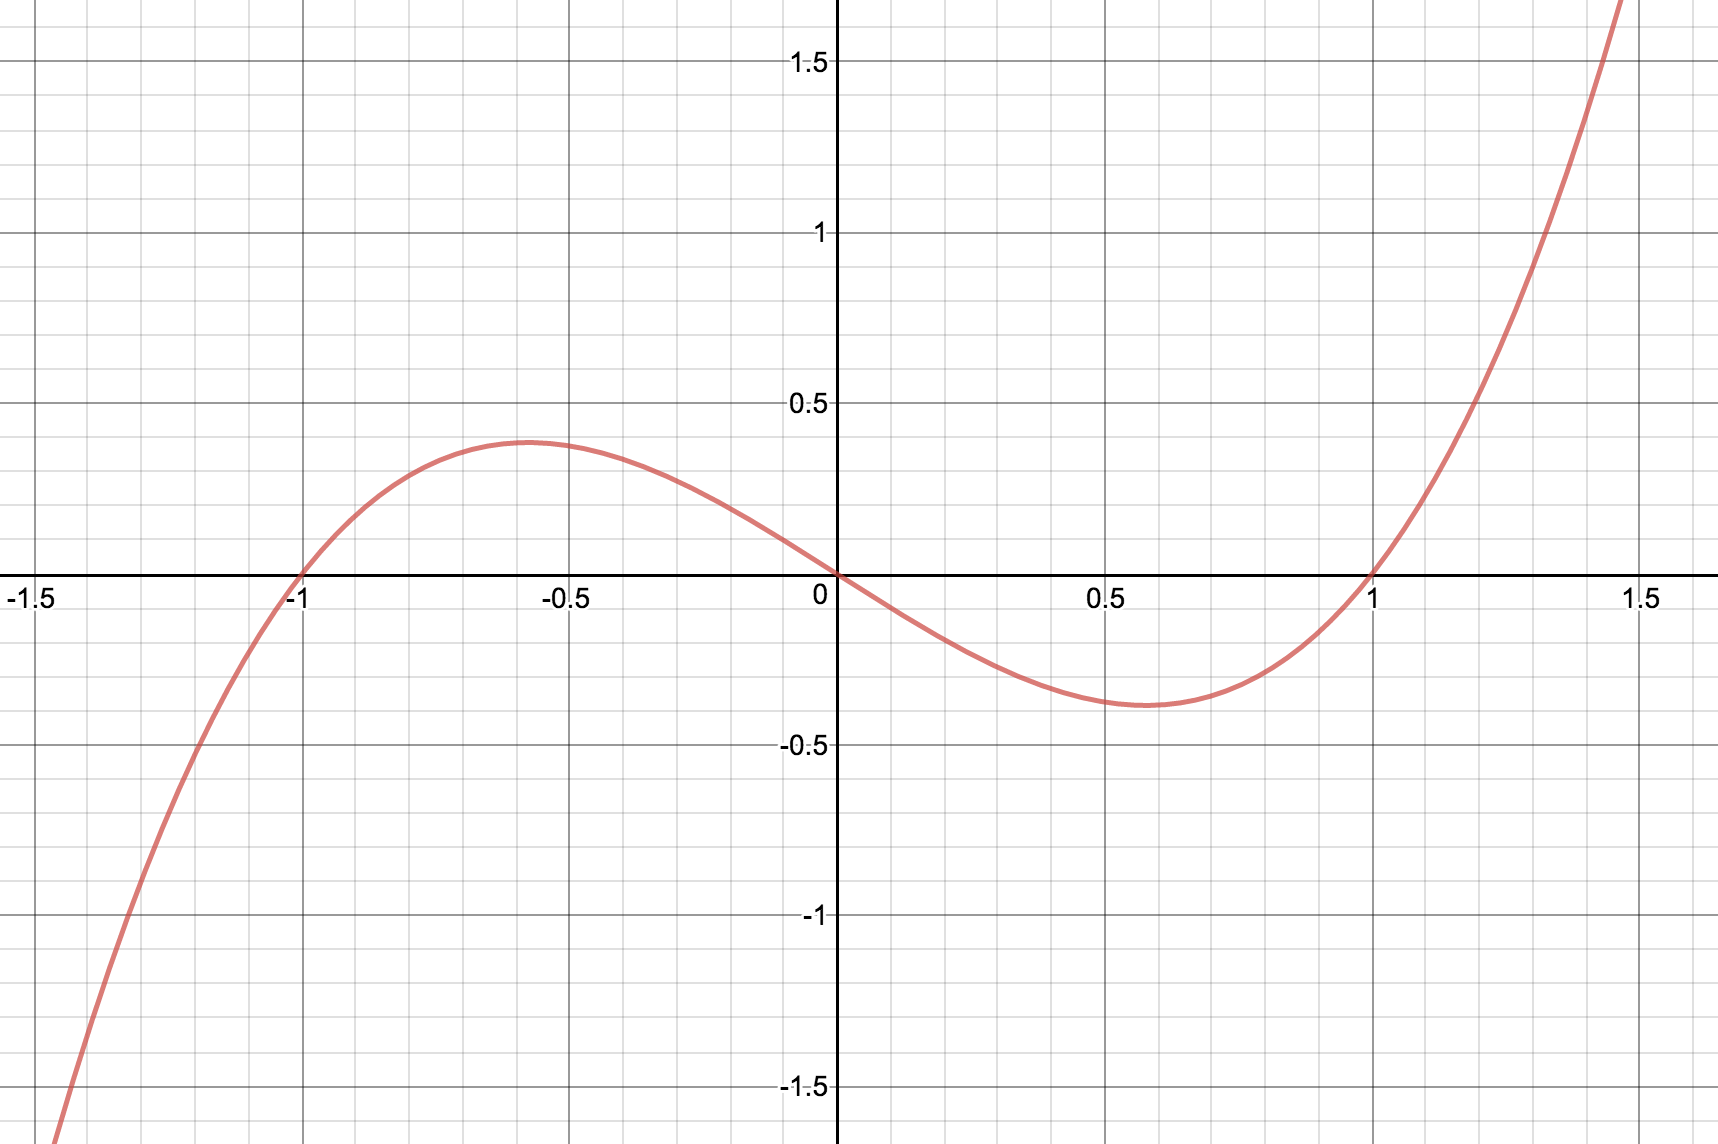
\includegraphics[width=4in]{poly.png}
  {\caption*{}}
  \label{}
\end{figure}
\section*{Bonus}
Find all roots of the polynomial $x^3-x^2+x-1$.  Explain why this example illustrates how the ``only real roots'' assumption simplifies the answer to the first part.

\newpage
\section*{Solution}
From the graph, you can see that the polynomial has roots at $x=-1$, $x=0$, and $x=1$.  Since the polynomial has only real roots, its equation must be $p(x) = (x - - 1)(x - 0)(x - 1) = x^3 - x$.

\section*{Bonus Solution}
$x^3 - x^2 + x - 1 = (x^2 + 1)(x - 1) = (x - i)(x -- i)(x - 1)$
This polynomial has roots at $\pm i$ in the complex plane and at the real number 1.  Its graph shows only the real root at $x = 1$.  So in general, just multiplying together $(x - r_i)$ where the $r_i$ are the real roots (what you can see in its graph) will not always give you the equation of the polynomial.  If you have all of the complex roots, it will always work (up to a constant). A beautiful fact about the Complex numbers is that they make up what is called an \textit{algebraically closed field} with the consequence that every polynomial of degree $n$ with real or complex coefficients can be factored into a product like the above, giving $n$ roots.  Some may be ``repeated'' as in $p(x) = x^2 = (x - 0)(x - 1)$.

\section*{Bonus Bonus Solution}
There is actually an error in the solution above. The graph is in fact the graph of the given function, but that can't actually be established from the information given.  If $p(x)$ is a polynomial and $c$ is a non-zero constant, the $r(x) = c \mathord{\cdot} p(x)$ is another polynomial with the same roots.  So for example, $2x^3 - 2x$ would also have the same roots as the polynomial above.
 
\end{document}

